% +------------------------------------------------------------------------+
% | CGAL Reference Manual:  Subdivision_surfaces_3
% +------------------------------------------------------------------------+
% | Subdivision surfaces on generic Polyhedron.
% | 
% | 1.2.2005  Le-Jeng Andy Shiue
% |
\RCSdef{\subdivisionRev}{$Revision$}
\RCSdefDate{\subdivisionDate}{$Date$}
% +------------------------------------------------------------------------+

\def\CC{Catmull-Clark}
\def\DS{Doo-Sabin}
\def\SQRT3{$\sqrt{3}$}
\def\SUB3{\ccc{Subdivision_surfaces_3}}

% ------------------------------------------------------------------------
\def\FIGDIR{Subdivision_surfaces_3/FIG}
\def\IL{{\itshape left}}
\def\IR{{\itshape right}}
\def\IM{{\itshape middle}}
\def\IT{{\itshape top}}
\def\IB{{\itshape bottom}}
% ------------------------------------------------------------------------

\ccParDims

\chapter{Subdivision Surfaces}
\label{chapterSubdivision}
\ccChapterRelease{\subdivisionRev. \ \subdivisionDate}
\ccChapterAuthor{Le-Jeng Andy Shiue}

%% \begin{ccTexOnly}
%%     \setlength{\unitlength}{1mm}
%%     \begin{picture}(0,0)(0.0,0.0)
%%       \put (78,25){% textwidth = 156mm
%%           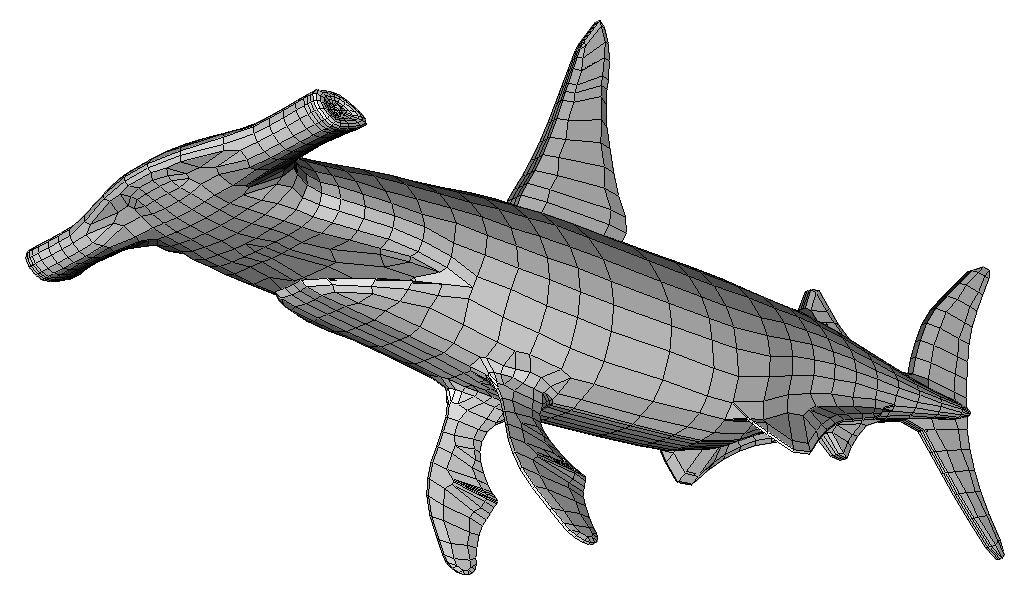
\includegraphics[width=0.5\textwidth]{Polyhedron/fig/shark}
%%       }
%%     \end{picture}\vspace{-4mm}% compensate for some vspace added by picture
%% \end{ccTexOnly}

\minitoc

% +------------------------------------------------------------------------+
\section{Introduction} \label{sectionSubIntro}
% +------------------------------------------------------------------------+
Subdivision algorithms (see e.g.\ \cite{Warren-2002-subdivision})
recursively refine coarse meshes
and generate ever closer approximations to a smooth surface.
%for character animation, surface modeling, or physics simulation. 
Setting aside the specific geometric placement strategy
for the new points, subdivision algorithms can be classified according to
the topological refinement of the underlying mesh.
\SUB3, based on the highly flexible design 
of the \ccc{CGAL::Polyhedron_3} (see Chapter~\ref{chapterPolyhedron}),
take advantage of this separation of connectivity and 
geometry and take a cue from the policy-based design.

 
%% \begin{ccHtmlOnly}
%%     <CENTER>
%%         <img src="./fig/shark.gif" alt="Hammerhead"><P>
%%     </CENTER>
%% \end{ccHtmlOnly}

%% the combinatorial integrity of them. It is based on the highly
%% flexible design of the halfedge data structure, see the introduction
%% in Chapter~\ref{chapterHalfedgeDS} and~\cite{k-ugpdd-99}. However, the
%% polyhedral surface can be used and understood with


% +------------------------------------------------------------------------+
\section{Subdivision Algorithms}
% +------------------------------------------------------------------------+
Subdivision algorithms define surfaces as the limit
of recursive refinement of a polyhedral mesh. 
%% A mesh is a special graph whose
%% primitives (i.e.~vertices, edges and facets)
%% carry attribute information such as vertex 
%% positions or facet colors. 
The mesh is recursively refined and then 
smoothed by averaging neighbors.
The four major refinement patterns used in practice
are shown in Figure \ref{fig:RefSchemes}.

A graph, called \emph{stencil}, determines the source submesh 
whose nodes contribute to the position of a target node.
For example, as illustrated in Figure \ref{fig:RefMap},
the PQQ scheme has a facet-node stencil,
an edge-node stencil and a vertex-node stencil 
while the DQQ scheme has only a corner-node stencil
(Figure \ref{fig:RefMap} \IR).
%% A stencil that includes only the vertices on facets that 
%% all share one node is called a \emph{1-ring}.
Stencils with weights are called \emph{geometry stencils}.
The geometry stencils for \CC\ subdivision are
shown in Figure \ref{fig:cc_gstencil}. The 
averaging step then positions points of the
refined mesh as a linear combination
of the points on the source submesh and the stencil weights.   
The averaging process can typically be factored into 
simpler steps \cite{Oswald-2003-CSS}.
%and this has
%been implemented in the OpenMesh library \cite{Sovakar-2004-APISUB}.
However, while stencil factoring simplifies the implementation,
it is less efficient because it requires repeated visits 
to all nodes.

\SUB3\ supports 1-ring mesh refinement based on 
half-edge data structures.
Since only a fixed number of \emph{abstract subdivision}
patterns (see Figure \ref{fig:RefSchemes}) are practical
but a wide variety of geometry stencils,
FSL provides abstract subdivisions (the hosts)
and hands the definition of \emph{concrete subdivisions}
(the policies) to the library user. A concrete 
subdivision (e.g.~\CC) is obtained by 
parameterizing the refinement host (PQQ refinement) 
with a geometry policy (\CC\ stencil).

A subdivision scheme of \ccc{CGAL::Subdivision_surfaces_3} is a 
refinement host parameterized with a geometry policy. The refinement
host realizes the connectivity refinement and the corresponding
stencils. The geometry policy consists a set of averaging rules
of the geometry stencils.

% +-------------------------------------------------------------+
\subsection{Example: \CC\ Subdivision}
\ccc{CGAL::Subdivision_surfaces_3::PQQ} is the refinement host of
the primal quadrilateral quadrisection.

\begin{ccExampleCode}
  // _S is the stencil policy
  template <template <typename> class _S>
  static void PQQ(Polyhedron& p, _S<Polyhedron> rule, int step)
\end{ccExampleCode}

\ccc{CGAL::CatmullClark_stencil} is the geometry policy of the
Catmull-Clark subdivision \cite{cc}. To subdivide a polyhedral
mesh, the \ccc{CGAL::Subdivision_surfaces_3::PQQ} is specialized
by \ccc{CGAL::CatmullClark_stencil}.

\begin{ccExampleCode}
  void CatmullClark_subdivision(Polyhedron& p, int step) {
    PQQ(p, CatmullClark_stencil<Polyhedron>(), step);
  }
\end{ccExampleCode}

Catmull-Clark, Loop, Doo-Sabin and $\sqrt{3}$ subdivisions are supported
in \ccc{CGAL::Subdivision_surfaces_3} as convenient functions.

% +-------------------------------------------------------------+
\section{Refinement Host}
\SUB3\ provides refinement hosts for subdivisions based on
primal quadrilateral quadrisection (PQQ), primal triangle 
quadrisection (PTQ), dual quadrilateral quadrisection (DQQ) and 
\SQRT3 triangulation, which are used by \CC, Loop, \DS\ and
\SQRT3\ subdivision, respectively. The refined mesh is shown below 
the initial mesh.

\begin{ccTexOnly}
  \begin{center}
    \parbox{0.6\textwidth}{%
      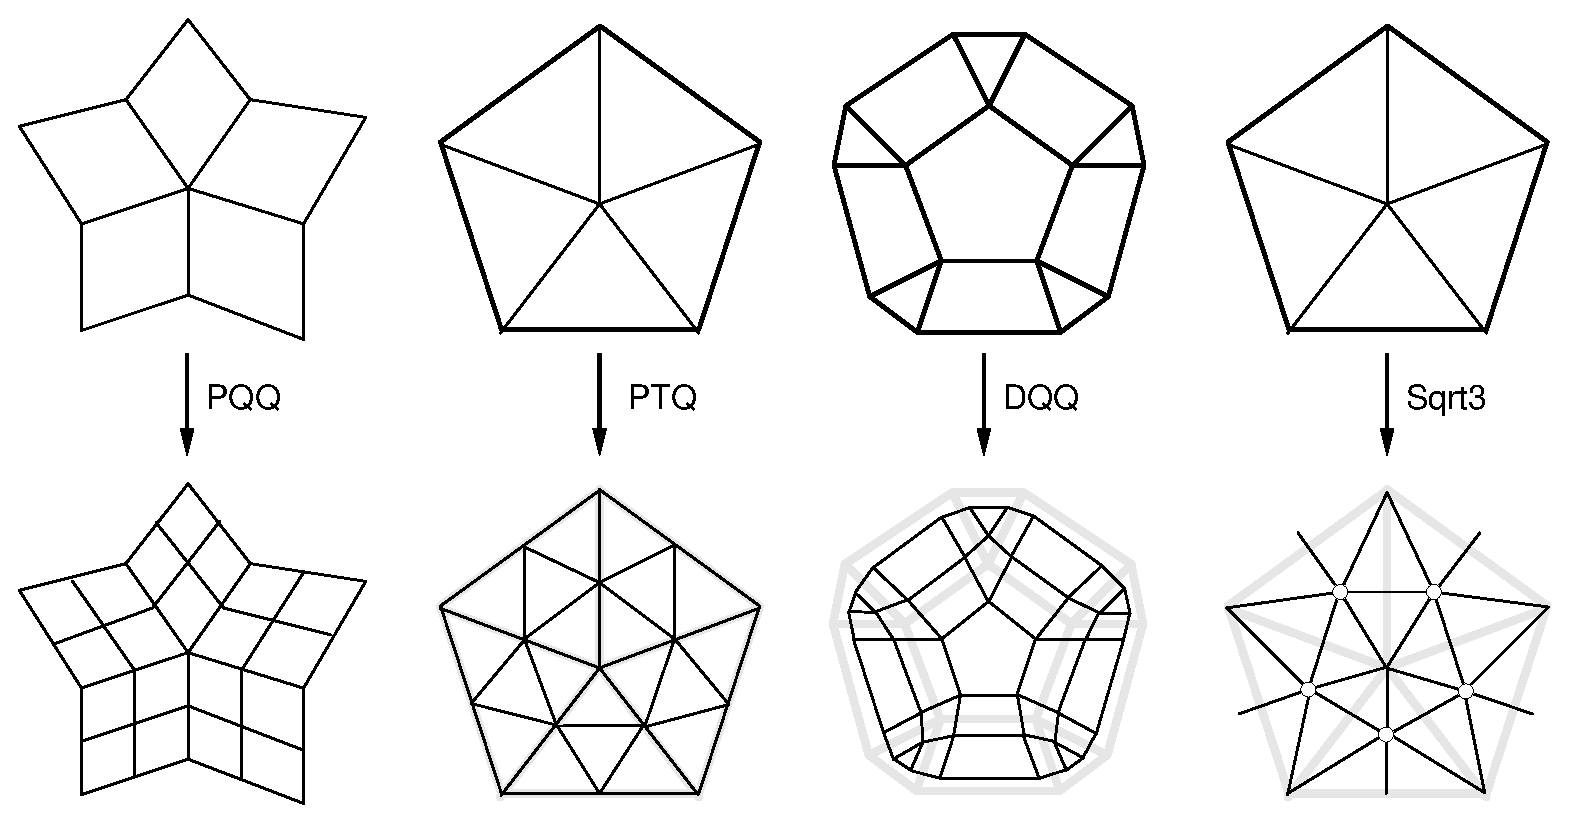
\includegraphics[width=0.6\textwidth]{\FIGDIR/RefSchemes.eps}%
    }
  \end{center}
\end{ccTexOnly}

\begin{ccHtmlOnly}
  <CENTER>
  <A HREF="./FIG/RefSchemes.gif">
     <img src="./FIG/RefSchemes.gif" alt="Refinement Hosts"></A><P>
  </CENTER>
\end{ccHtmlOnly}

%% Stencils are maintained using the iteration concept
%% to avoid the need for vertex tags to distinguish
%% the stencil types.
%% For example, on a PQQ refined mesh, the vertex iterator 
%% visits the 
%% vertex-nodes, edge-nodes and then facet-nodes. The visit
%% order is implicitly used to determine the stencil of
%% the visited node.

Each refinement host is realized as a static function of
the refining polyhedron mesh and the geometry policy. 

\begin{ccExampleCode}
template <class Polyhedron>
class Subdivision_surfaces_3 {
  // _S is the stencil policy
  template <template <typename> class _S>
  static void PQQ(Polyhedron& p, _S<Polyhedron> rule, int step);

  template <template <typename> class _S>
  static void PTQ(Polyhedron& p, _S<Polyhedron> rule, int step);

  template <template <typename> class _S>
  static void DQQ(Polyhedron& p, _S<Polyhedron> rule, int step);

  template <template <typename> class _S>
  static void Sqrt3(Polyhedron& p, _S<Polyhedron> rule, int step);
}
\end{ccExampleCode}

% +-------------------------------------------------------------+
\section{Geometry Policy}
A geometry policy defines a set of functions of the geometry stencil.
The policy interface is defined with the refinement host. Each policy 
function receives a primitive handle of the source polyhedral mesh,
and the target node as the reference of the \ccc{Point}.
A concrete policy function is semantically required to assigned 
the smoothed point based on the source mesh.

A PQQ reinement host requires three policies for a closed surface.
\begin{ccTexOnly}
  \begin{center}
    \parbox{0.5\textwidth}{%
      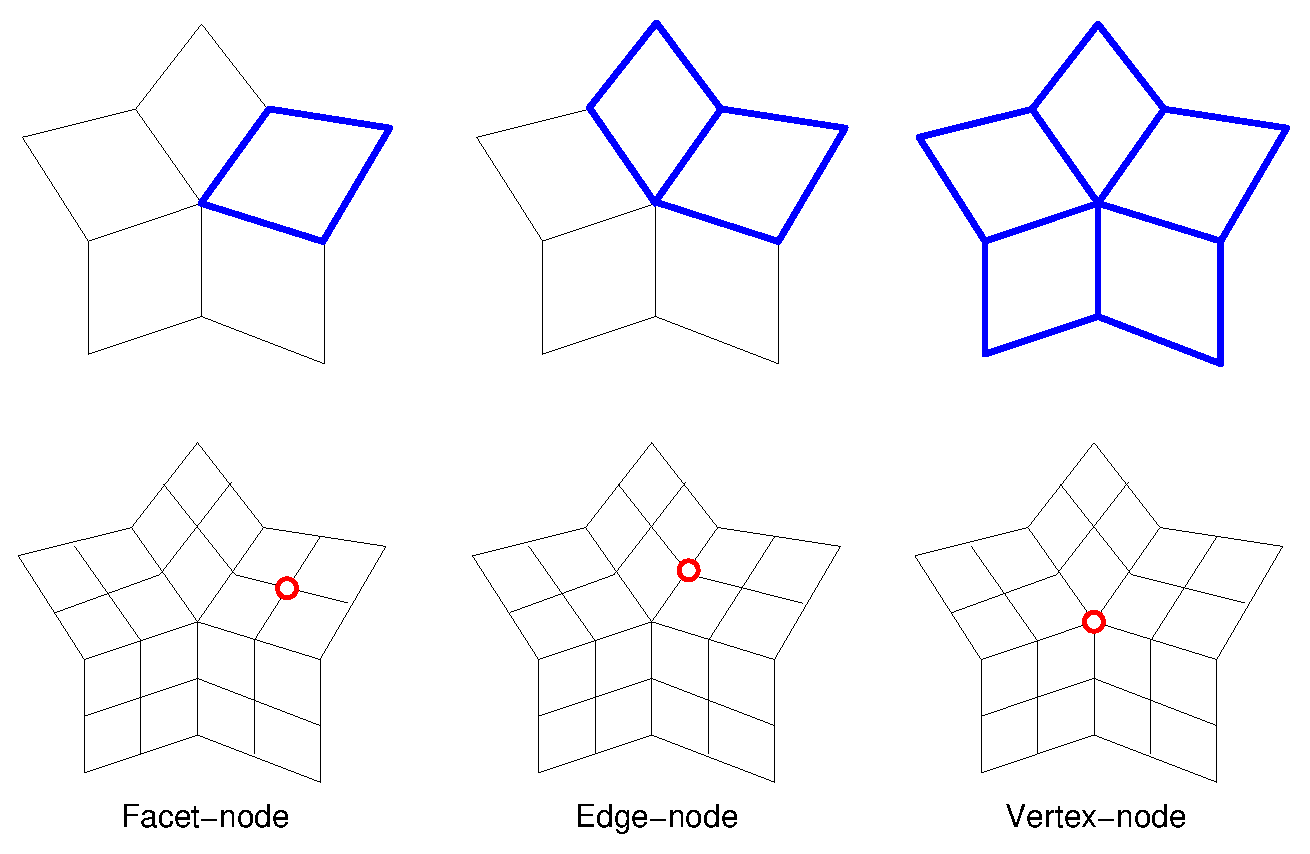
\includegraphics[width=0.5\textwidth]{\FIGDIR/PQQStencil.eps}%
    }
  \end{center}
\end{ccTexOnly}

\begin{ccHtmlOnly}
  <CENTER>
  <A HREF="./FIG/PQQStencil.gif">
     <img src="./FIG/PQQStencil.gif" alt="Stecils of PQQ scheme "></A><P>
  </CENTER>
\end{ccHtmlOnly}

Following shows the realization of the \CC\ rules as the geometry policy.
To support the border, an additional policy for border vertices is 
required.
\begin{ccExampleCode}
template <class _Poly>
class CatmullClark_stencil {
   void edge_node(Halfedge_handle edge, Point& pt) {
    Point p1 = edge->vertex()->point();
    Point p2 = edge->opposite()->vertex()->point();
    Point f1, f2;
    facet_node(edge->facet(), f1);
    facet_node(edge->opposite()->facet(), f2);
    pt = Point((p1[0]+p2[0]+f1[0]+f2[0])/4,
               (p1[1]+p2[1]+f1[1]+f2[1])/4,
               (p1[2]+p2[2]+f1[2]+f2[2])/4 );
  }
 
  void vertex_node(Vertex_handle vertex, Point& pt) {
    Halfedge_around_vertex_circulator vcir = vertex->vertex_begin();
    int n = circulator_size(vcir);    

    float Q[] = {0.0, 0.0, 0.0}, R[] = {0.0, 0.0, 0.0};
    Point& S = vertex->point();
    
    Point q;
    for (int i = 0; i < n; i++, ++vcir) {
      Point& p2 = vcir->opposite()->vertex()->point();
      R[0] += (S[0]+p2[0])/2;
      R[1] += (S[1]+p2[1])/2;
      R[2] += (S[2]+p2[2])/2;
      facet_node(vcir->facet(), q);
      Q[0] += q[0];      
      Q[1] += q[1];      
      Q[2] += q[2];
    }
    R[0] /= n;    R[1] /= n;    R[2] /= n;
    Q[0] /= n;    Q[1] /= n;    Q[2] /= n;
      
    pt = Point((Q[0] + 2*R[0] + S[0]*(n-3))/n,
               (Q[1] + 2*R[1] + S[1]*(n-3))/n,
               (Q[2] + 2*R[2] + S[2]*(n-3))/n );
  }

  void border_node(Halfedge_handle edge, Point& ept, Point& vpt) {
    Point& ep1 = edge->vertex()->point();
    Point& ep2 = edge->opposite()->vertex()->point();
    ept = Point((ep1[0]+ep2[0])/2, (ep1[1]+ep2[1])/2, (ep1[2]+ep2[2])/2);

    Halfedge_around_vertex_circulator vcir = edge->vertex_begin();
    Point& vp1  = vcir->opposite()->vertex()->point();
    Point& vp0  = vcir->vertex()->point();
    Point& vp_1 = (--vcir)->opposite()->vertex()->point();
    vpt = Point((vp_1[0] + 6*vp0[0] + vp1[0])/8,
                (vp_1[1] + 6*vp0[1] + vp1[1])/8,
                (vp_1[2] + 6*vp0[2] + vp1[2])/8 );
  }
}
\end{ccExampleCode}

%% \begin{ccExampleCode}
%% PQQ<_M,CCstencil>(Mesh,CCstencil<_M>())
%% \end{ccExampleCode}
%% (or, more simply \\
%% \begin{ccExampleCode}
%% PQQ(Mesh,CCstencil<_M>())}
%% \end{ccExampleCode}
%% since the compiler can derive the template
%% arguments from the function parameters),
%% instantiates \CC\ subdivision.    
%% \ccc{_M}, the model of the mesh concept,
%% represents the mesh type (\ccc{Mesh}),
%% and \ccc{CCstencil} is a class template 
%% realizing geometry policies of \CC\ subdivision.

The geometry stencil of \CC\ subdivision (border rules is not included) 
is shown below. 

\begin{ccTexOnly}
  \begin{center}
    \parbox{0.4\textwidth}{%
      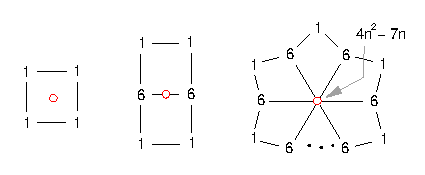
\includegraphics[width=0.4\textwidth]{\FIGDIR/cc_mask.eps}%
    }
  \end{center}
\end{ccTexOnly}

\begin{ccHtmlOnly}
  <CENTER>
  <A HREF="./FIG/cc_mask.gif">
     <img src="./FIG/cc_mask.gif" alt="\CC\ geometry stencil"></A><P>
  </CENTER>
\end{ccHtmlOnly}


% +------------------------------------------------------------------------+
\section{Bult-in subdivisions}
% +------------------------------------------------------------------------+
\CC , Loop, \DS\ and \SQRT3\ subdivisions are provided in \SUB3. Each of these 
subdivision schemes is instantiated with the corresponding geometry policy.
\begin{ccExampleCode}
  static void CatmullClark_subdivision(Polyhedron& p, int step) {
    PQQ(p, CatmullClark_stencil<Polyhedron>(), step);
  }
  static void Loop_subdivision(Polyhedron& p, int step) {
    PTQ(p, Loop_stencil<Polyhedron>() , step);
  }
  static void DooSabin_subdivision(Polyhedron& p, int step) {
    DQQ(p, DooSabin_stencil<Polyhedron>(), step);
  }
  static void Sqrt3_subdivision(Polyhedron& p, int step) {
    Sqrt3(p, Sqrt3_stencil<Polyhedron>(), step);
  }
\end{ccExampleCode}

Following shows an example of \DS\ subdivision on a polyhedral mesh.
\ccIncludeExampleCode{Subdivision_surfaces_3/DooSabin_subdivision.C}

% +------------------------------------------------------------------------+
\section{Create your own subdivision surfaces}
% +------------------------------------------------------------------------+
To create a user-defined subdivision, you need to choose a refinement host 
(e.g.~\ccc{Subdivision_surfaces_3<Polyhedron>::PTQ}) and implement the
geometry policy accordingly (e.g.~a subclass of \ccc{PTQ_stencil}). 
\ccIncludeExampleCode{Subdivision_surfaces_3/Customized_subdivision.C}
